\subsection{Jockey Dashboard}
\subsubsection{Class Diagram}

\begin{figure}[H]
    \centering
    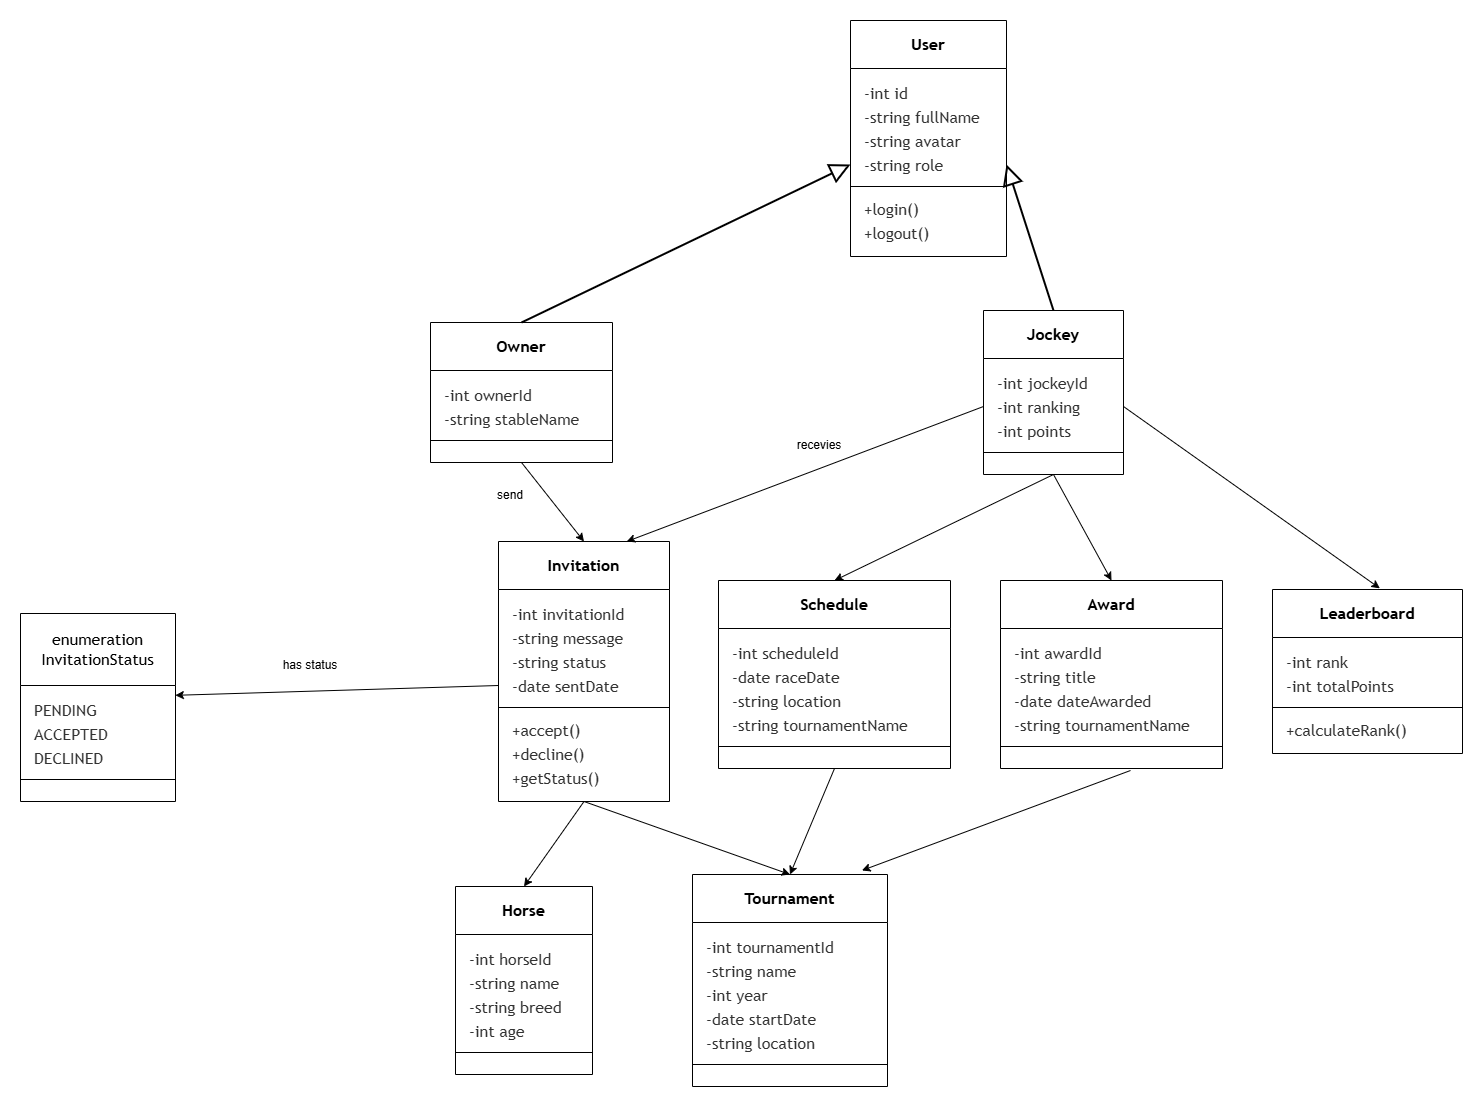
\includegraphics[width=\textwidth,height=0.78\textheight,keepaspectratio]{figures/design/Jockey/classdiagram_jockey_dashborad.drawio.png}
    \caption{Jockey Dashboard Class Diagram}
    \label{fig:jockey_dashboard_class_diagram}
\end{figure}

\subsubsection{Sequence Diagram}

\begin{figure}[H]
    \centering
    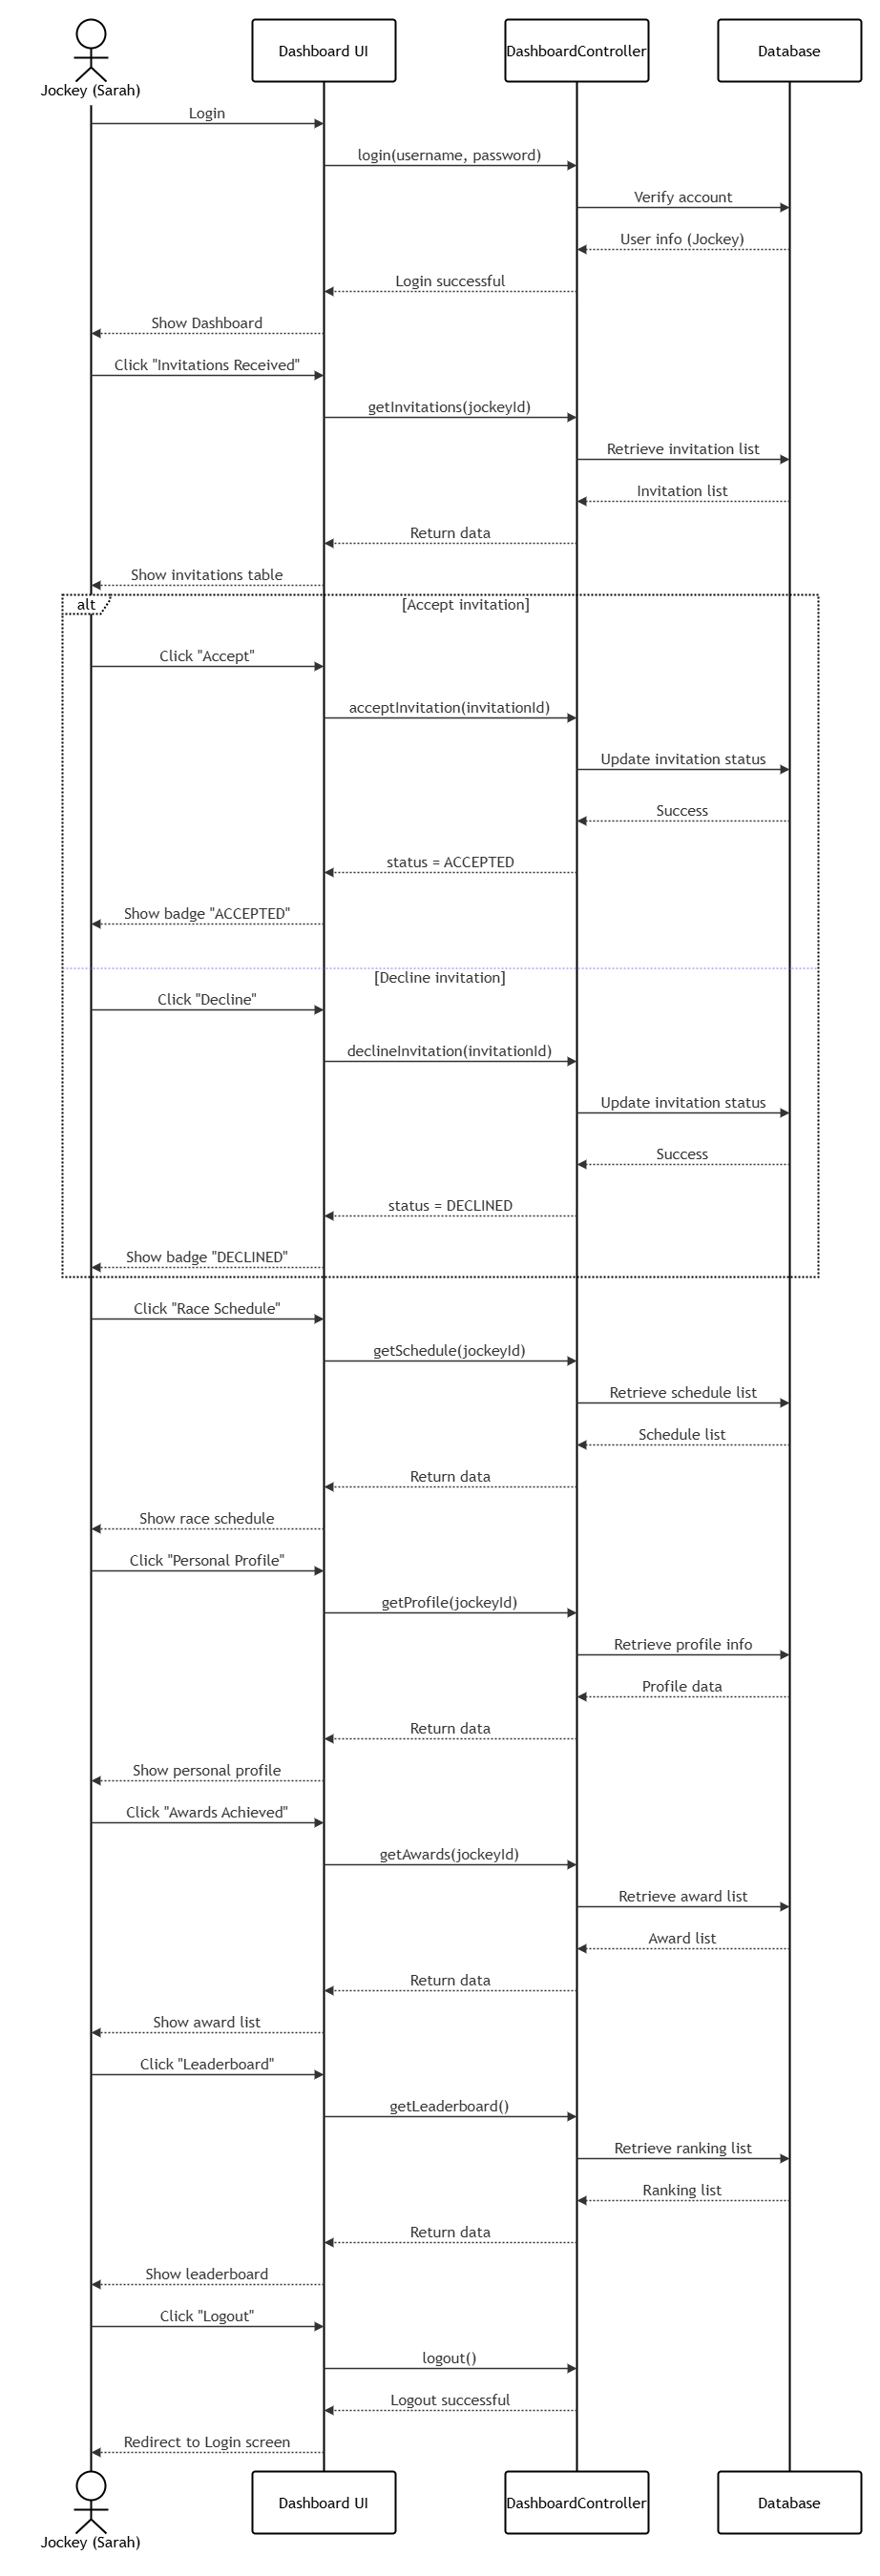
\includegraphics[width=\textwidth,height=0.78\textheight,keepaspectratio]{figures/design/Jockey/Sequence_jockey_dashborad.png}
    \caption{Jockey Dashboard Sequence Diagram}
    \label{fig:jockey_dashboard_sequence_diagram}
\end{figure}

\subsubsection{Class Specification}

\begingroup
\small
\setlength{\tabcolsep}{3pt}
\begin{longtable}{|>{\raggedright\arraybackslash}p{0.16\textwidth}|>{\raggedright\arraybackslash}p{0.30\textwidth}|>{\raggedright\arraybackslash}p{0.14\textwidth}|>{\raggedright\arraybackslash}p{0.25\textwidth}|}
\caption{Jockey Dashboard class specification}
\label{tab:jockey_dashboard_class_spec} \\
\hline
\tableHeader
\textbf{Class} & \textbf{Attributes / Methods} & \textbf{Type} & \textbf{Description} \\
\hline
\endfirsthead
\hline
\tableHeader
\textbf{Class} & \textbf{Attributes / Methods} & \textbf{Type} & \textbf{Description} \\
\hline
\endhead
User & id, fullName, avatar, role, login(), logout() & entity & Represents the base account of a system user. Both \texttt{Owner} and \texttt{Jockey} inherit from this class. \\
\hline
Jockey & jockeyId, ranking, points & entity & Extends \texttt{User} with jockey-specific attributes; linked to invitations, schedules, awards, and the leaderboard. \\
\hline
Owner & ownerId, stableName & entity & Extends \texttt{User} and sends invitations to jockeys on behalf of a stable. \\
\hline
Invitation & invitationId, message, status, sentDate, accept(), decline(), getStatus() & entity & Records a race invitation sent by an owner to a jockey, with the current status tracked via \texttt{InvitationStatus}. \\
\hline
Invitation\allowbreak{}Status & PENDING, ACCEPTED, DECLINED & enumeration & Enumerates the possible lifecycle states of a jockey invitation. \\
\hline
Schedule & scheduleId, raceDate, location, tournamentName & entity & Stores race schedule details visible to the jockey after an invitation is accepted. \\
\hline
Award & awardId, title, dateAwarded, tournamentName & entity & Records awards and achievements earned by the jockey in tournaments. \\
\hline
Leaderboard & rank, totalPoints, calculateRank() & entity & Maintains the global jockey ranking and calculates each jockey's position based on accumulated points. \\
\hline
Horse & horseId, name, breed, age & entity & Represents the horse assigned to a jockey through an invitation for a specific tournament. \\
\hline
Tournament & tournamentId, name, year, startDate, location & entity & Represents the racing tournament context that links invitations, schedules, and awards together. \\
\hline
Dashboard\allowbreak{}UI & login(), getInvitations(), acceptInvitation(), declineInvitation(), getSchedule(), getProfile(), getAwards(), getLeaderboard(), logout() & boundary / UI & The jockey-facing dashboard interface that handles login, displays invitations, schedule, profile, awards, and the leaderboard. \\
\hline
Dashboard\allowbreak{}Controller & login(username, password), getInvitations(jockeyId), acceptInvitation(invitationId), declineInvitation(invitationId), getSchedule(jockeyId), getProfile(jockeyId), getAwards(jockeyId), getLeaderboard() & controller & Processes all dashboard requests from the UI, coordinates data retrieval and status updates with the database. \\
\hline
\end{longtable}

\subsection{Jockey Invitation Management}
\subsubsection{Class Diagram}

\begin{figure}[H]
    \centering
    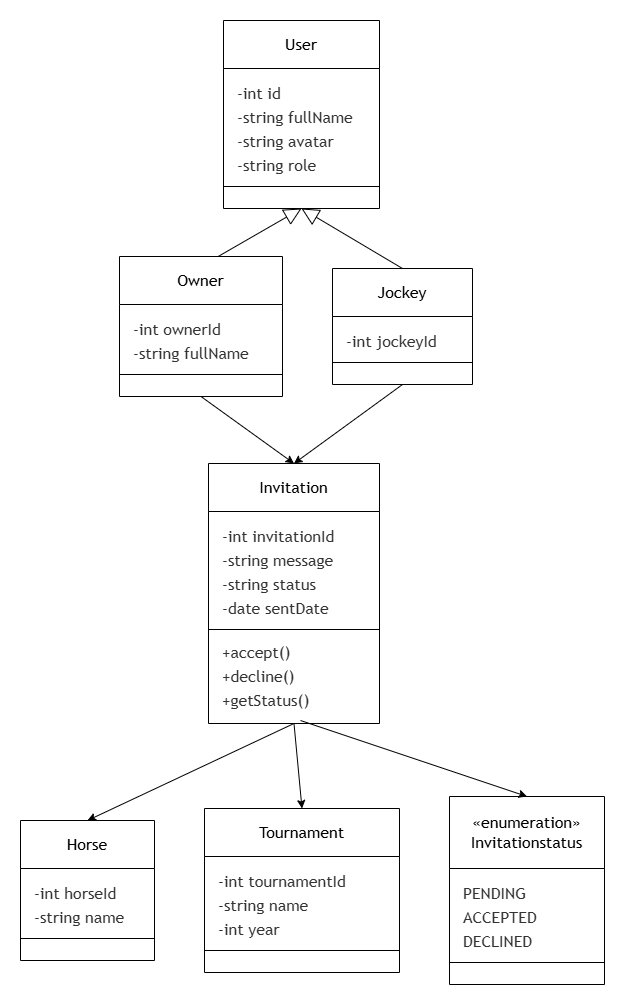
\includegraphics[width=\textwidth,height=0.78\textheight,keepaspectratio]{figures/design/Jockey/classdiagram_jockey_invite.drawio.png}
    \caption{Jockey Invitation Management Class Diagram}
    \label{fig:jockey_invitation_class_diagram}
\end{figure}

\subsubsection{Sequence Diagram}

\begin{figure}[H]
    \centering
    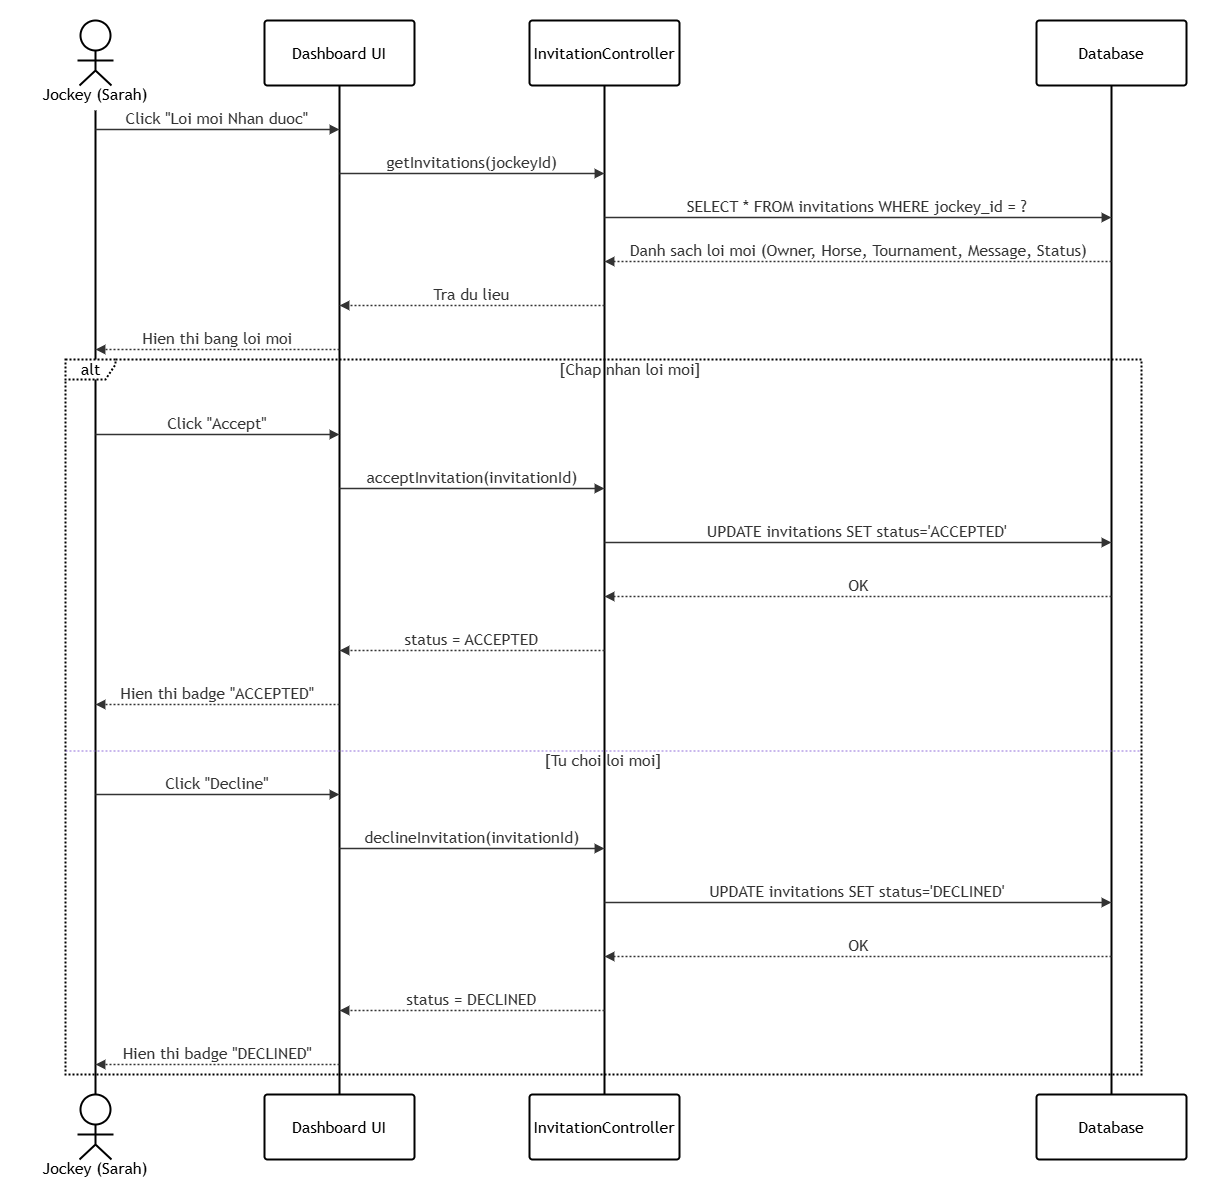
\includegraphics[width=\textwidth,height=0.78\textheight,keepaspectratio]{figures/design/Jockey/Sequence_jockey_invite.drawio.png}
    \caption{Jockey Invitation Management Sequence Diagram}
    \label{fig:jockey_invitation_sequence_diagram}
\end{figure}

\subsubsection{Class Specification}

\begingroup
\small
\setlength{\tabcolsep}{3pt}
\begin{longtable}{|>{\raggedright\arraybackslash}p{0.16\textwidth}|>{\raggedright\arraybackslash}p{0.30\textwidth}|>{\raggedright\arraybackslash}p{0.14\textwidth}|>{\raggedright\arraybackslash}p{0.25\textwidth}|}
\caption{Jockey Invitation Management class specification}
\label{tab:jockey_invitation_class_spec} \\
\hline
\tableHeader
\textbf{Class} & \textbf{Attributes / Methods} & \textbf{Type} & \textbf{Description} \\
\hline
\endfirsthead
\hline
\tableHeader
\textbf{Class} & \textbf{Attributes / Methods} & \textbf{Type} & \textbf{Description} \\
\hline
\endhead
User & id, fullName, avatar, role & entity & Base account class inherited by both \texttt{Owner} and \texttt{Jockey}; provides shared identity attributes. \\
\hline
Owner & ownerId, fullName & entity & Extends \texttt{User}; represents the horse owner who sends race invitations to jockeys. \\
\hline
Jockey & jockeyId & entity & Extends \texttt{User}; represents the jockey who receives and responds to invitations. \\
\hline
Invitation & invitationId, message, status, sentDate, accept(), decline(), getStatus() & entity & Records the invitation sent from an owner to a jockey, supporting accept and decline actions with status tracking. \\
\hline
Invitation\allowbreak{}Status & PENDING, ACCEPTED, DECLINED & enumeration & Defines the three possible lifecycle states of a jockey invitation. \\
\hline
Horse & horseId, name & entity & Represents the horse associated with the invitation that the jockey is being asked to ride. \\
\hline
Tournament & tournamentId, name, year & entity & Provides the tournament context for the invitation, linking the jockey and horse to a specific racing event. \\
\hline
Dashboard\allowbreak{}UI & getInvitations(jockeyId), acceptInvitation(invitationId), declineInvitation(invitationId) & boundary / UI & Displays the invitation list to the jockey and handles accept and decline user interactions. \\
\hline
Invitation\allowbreak{}Controller & getInvitations(jockeyId), acceptInvitation(invitationId), declineInvitation(invitationId) & controller & Processes invitation retrieval and status update requests, coordinates between the UI and the database. \\
\hline
\end{longtable}
\endgroup

\subsection{Race Schedule}
\subsubsection{Class Diagram}

\begin{figure}[H]
    \centering
    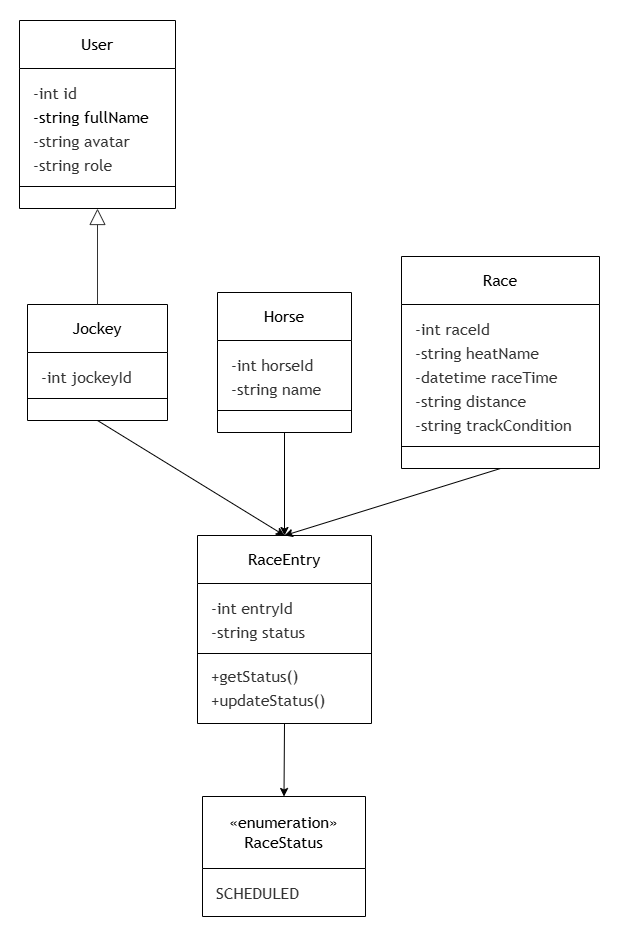
\includegraphics[width=\textwidth,height=0.78\textheight,keepaspectratio]{figures/design/Jockey/classdiagram_jockey_chedule.drawio.png}
    \caption{Race Schedule Class Diagram}
    \label{fig:jockey_schedule_class_diagram}
\end{figure}

\subsubsection{Sequence Diagram}

\begin{figure}[H]
    \centering
    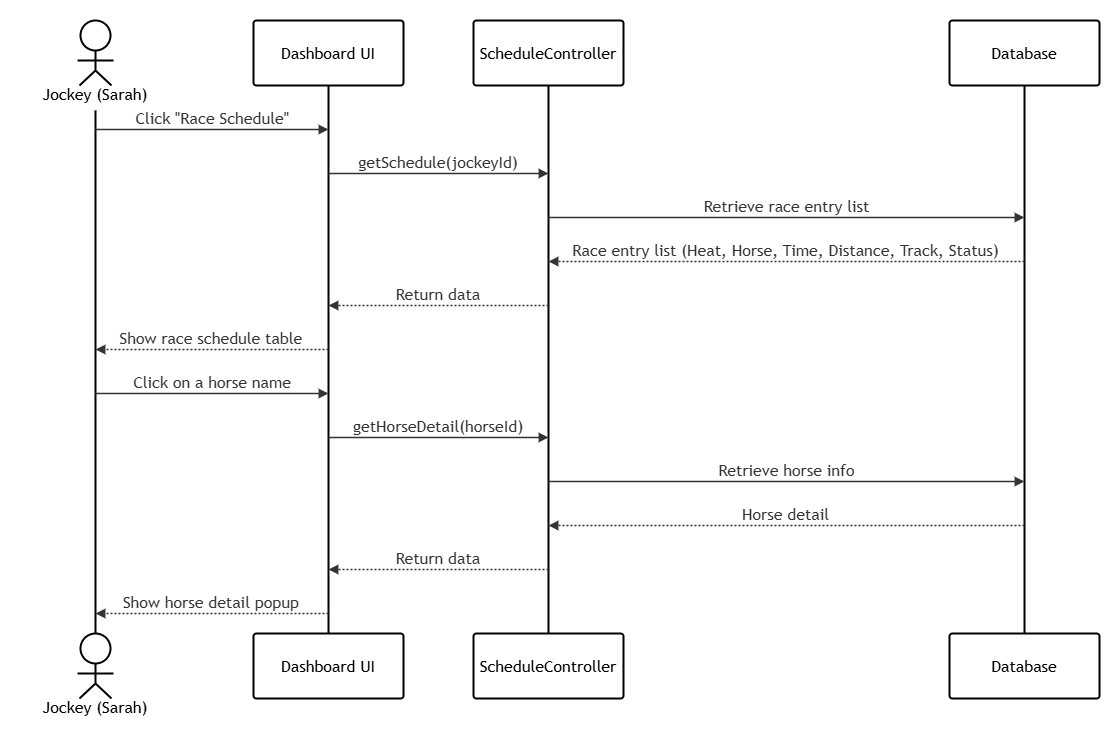
\includegraphics[width=\textwidth,height=0.78\textheight,keepaspectratio]{figures/design/Jockey/sequence_jockey_chedule.drawio.png}
    \caption{Race Schedule Sequence Diagram}
    \label{fig:jockey_schedule_sequence_diagram}
\end{figure}

\subsubsection{Class Specification}

\begingroup
\small
\setlength{\tabcolsep}{3pt}
\begin{longtable}{|>{\raggedright\arraybackslash}p{0.16\textwidth}|>{\raggedright\arraybackslash}p{0.30\textwidth}|>{\raggedright\arraybackslash}p{0.14\textwidth}|>{\raggedright\arraybackslash}p{0.25\textwidth}|}
\caption{Race Schedule class specification}
\label{tab:jockey_schedule_class_spec} \\
\hline
\tableHeader
\textbf{Class} & \textbf{Attributes / Methods} & \textbf{Type} & \textbf{Description} \\
\hline
\endfirsthead
\hline
\tableHeader
\textbf{Class} & \textbf{Attributes / Methods} & \textbf{Type} & \textbf{Description} \\
\hline
\endhead
User & id, fullName, avatar, role & entity & Base account class; \texttt{Jockey} inherits from it to access the race schedule feature. \\
\hline
Jockey & jockeyId & entity & Extends \texttt{User}; the authenticated jockey whose assigned race entries are retrieved and displayed. \\
\hline
Horse & horseId, name & entity & Represents the horse assigned to the jockey for a specific race entry. \\
\hline
Race & raceId, heatName, raceTime, distance, trackCondition & entity & Stores the details of an individual race heat, including time, distance, and track conditions. \\
\hline
Race\allowbreak{}Entry & entryId, status, getStatus(), updateStatus() & entity & Links a jockey and a horse to a specific race; tracks the entry status via \texttt{RaceStatus}. \\
\hline
Race\allowbreak{}Status & SCHEDULED & enumeration & Enumerates the status values of a race entry; currently supports the \texttt{SCHEDULED} state. \\
\hline
Dashboard\allowbreak{}UI & getSchedule(jockeyId), getHorseDetail(horseId) & boundary / UI & Renders the race schedule table and displays a horse detail popup when the jockey clicks a horse name. \\
\hline
Schedule\allowbreak{}Controller & getSchedule(jockeyId), getHorseDetail(horseId) & controller & Retrieves the list of race entries for the jockey and fetches detailed horse information on demand. \\
\hline
\end{longtable}
\endgroup

\subsection{Personal Profile}
\subsubsection{Class Diagram}

\begin{figure}[H]
    \centering
    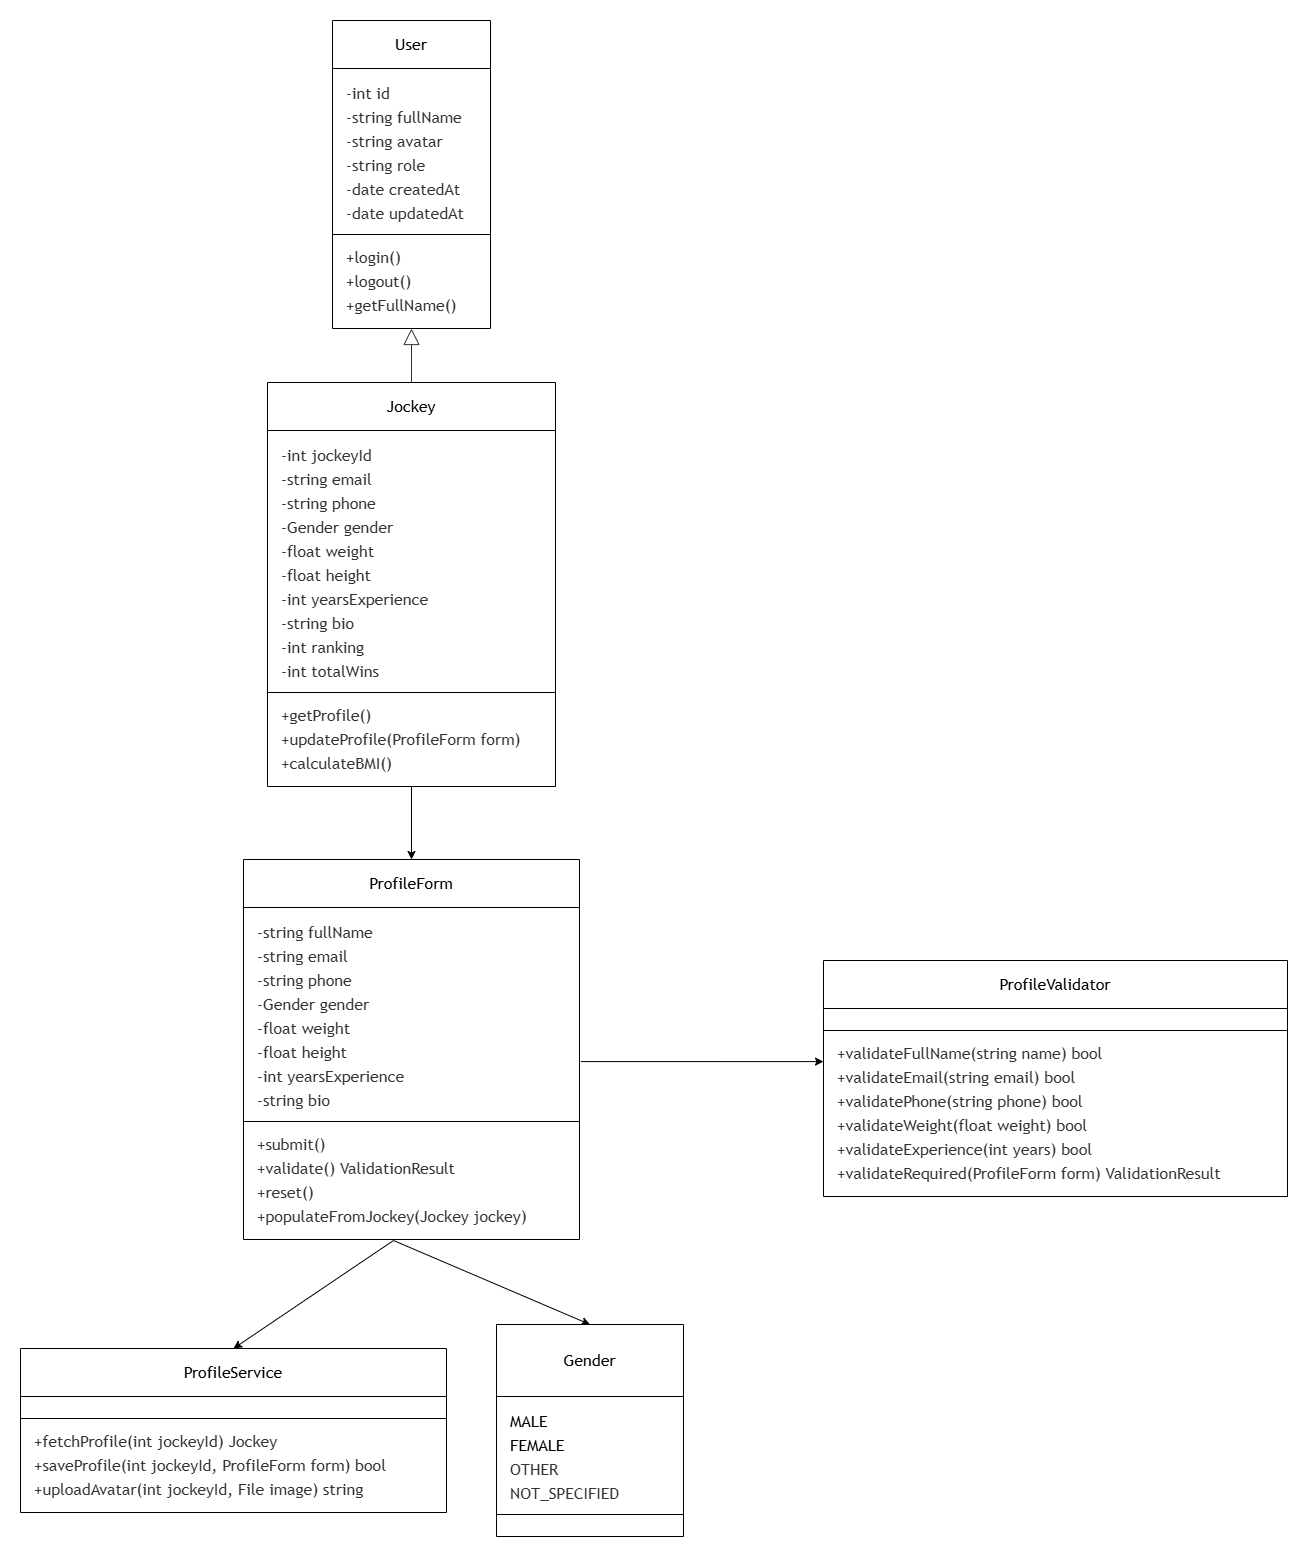
\includegraphics[width=\textwidth,height=0.78\textheight,keepaspectratio]{figures/design/Jockey/classdiagram_jockey_profile.drawio.drawio.png}
    \caption{Personal Profile Class Diagram}
    \label{fig:jockey_profile_class_diagram}
\end{figure}

\subsubsection{Sequence Diagram}

\begin{figure}[H]
    \centering
    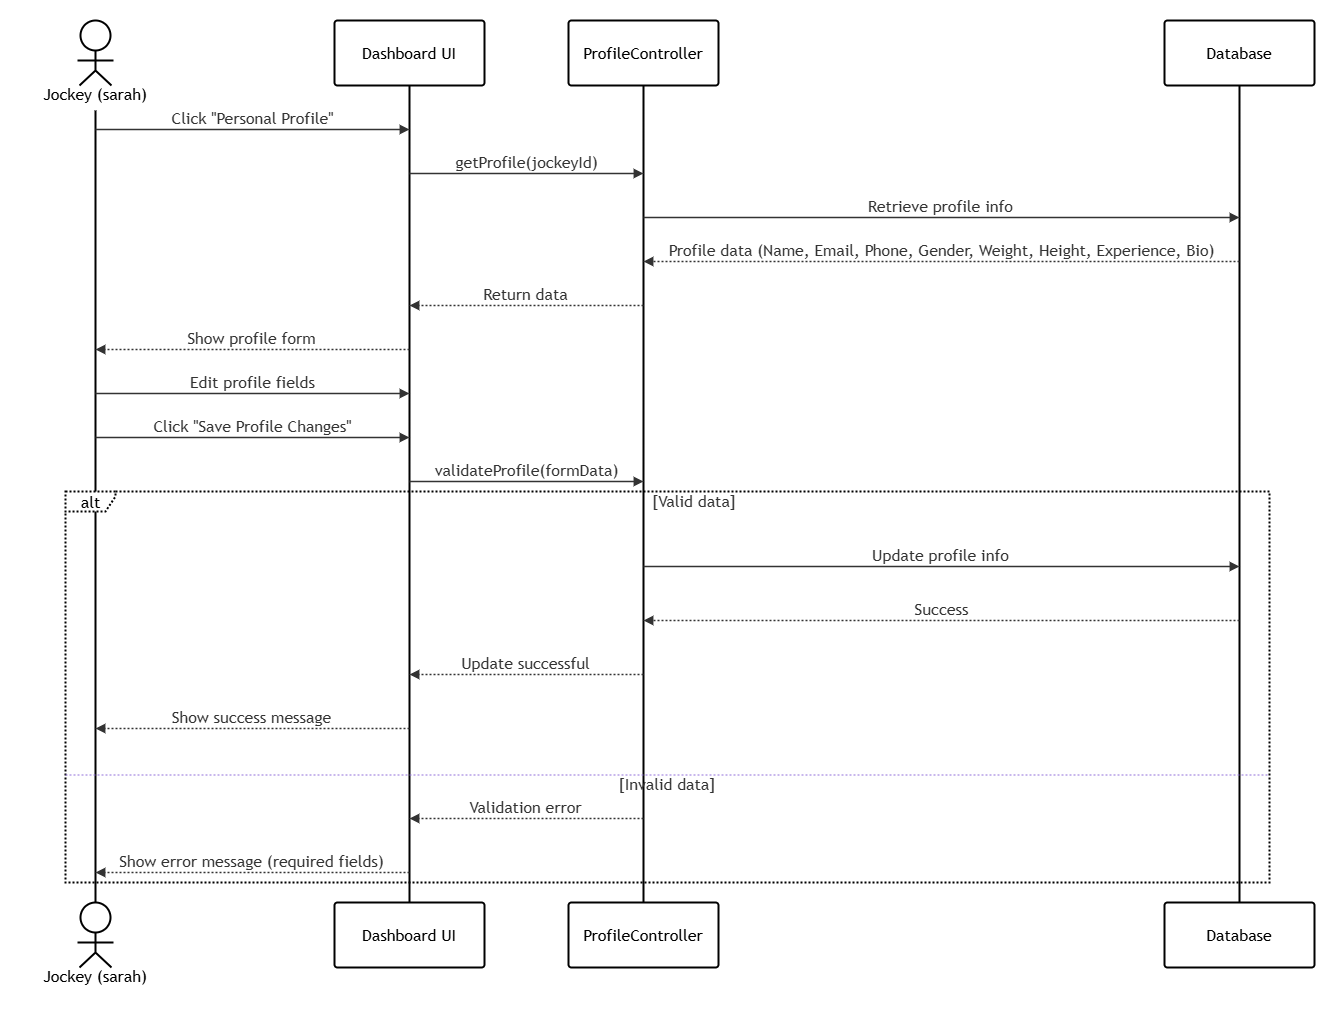
\includegraphics[width=\textwidth,height=0.78\textheight,keepaspectratio]{figures/design/Jockey/sequence_jockey_profile.drawio.png}
    \caption{Personal Profile Sequence Diagram}
    \label{fig:jockey_profile_sequence_diagram}
\end{figure}

\subsubsection{Class Specification}

\begingroup
\small
\setlength{\tabcolsep}{3pt}
\begin{longtable}{|>{\raggedright\arraybackslash}p{0.16\textwidth}|>{\raggedright\arraybackslash}p{0.30\textwidth}|>{\raggedright\arraybackslash}p{0.14\textwidth}|>{\raggedright\arraybackslash}p{0.25\textwidth}|}
\caption{Personal Profile class specification}
\label{tab:jockey_profile_class_spec} \\
\hline
\tableHeader
\textbf{Class} & \textbf{Attributes / Methods} & \textbf{Type} & \textbf{Description} \\
\hline
\endfirsthead
\hline
\tableHeader
\textbf{Class} & \textbf{Attributes / Methods} & \textbf{Type} & \textbf{Description} \\
\hline
\endhead
User & id, fullName, avatar, role, createdAt, updatedAt, login(), logout(), getFullName() & entity & Base account class providing core identity and authentication methods inherited by \texttt{Jockey}. \\
\hline
Jockey & jockeyId, email, phone, gender, weight, height, yearsExperience, bio, ranking, totalWins, getProfile(), updateProfile(ProfileForm), calculateBMI() & entity & Extends \texttt{User} with jockey-specific profile attributes; supports profile retrieval, update, and BMI calculation. \\
\hline
Profile\allowbreak{}Form & fullName, email, phone, gender, weight, height, yearsExperience, bio, submit(), validate(), reset(), populateFromJockey(Jockey) & DTO / form & Carries the form data submitted by the jockey when editing their personal profile, and validates required fields before saving. \\
\hline
Profile\allowbreak{}Validator & validateFullName(name), validateEmail(email), validatePhone(phone), validateWeight(weight), validateExperience(years), validateRequired(ProfileForm) & service & Validates individual profile fields and the entire form, returning a \texttt{ValidationResult} for each check. \\
\hline
Profile\allowbreak{}Service & fetchProfile(jockeyId), saveProfile(jockeyId, ProfileForm), uploadAvatar(jockeyId, image) & service & Handles backend communication for loading the jockey profile, persisting updates, and uploading avatar images. \\
\hline
Gender & MALE, FEMALE, OTHER, NOT\_SPECIFIED & enumeration & Defines the gender options available when the jockey edits their personal profile. \\
\hline
Dashboard\allowbreak{}UI & getProfile(jockeyId), validateProfile(formData) & boundary / UI & Displays the profile form pre-filled with existing data, handles edit interactions, and shows success or validation error messages. \\
\hline
Profile\allowbreak{}Controller & getProfile(jockeyId), validateProfile(formData) & controller & Retrieves profile data from the database and processes profile update requests, delegating validation to \texttt{ProfileValidator}. \\
\hline
\end{longtable}
\endgroup

\subsection{Achievements}
\subsubsection{Class Diagram}

\begin{figure}[H]
    \centering
    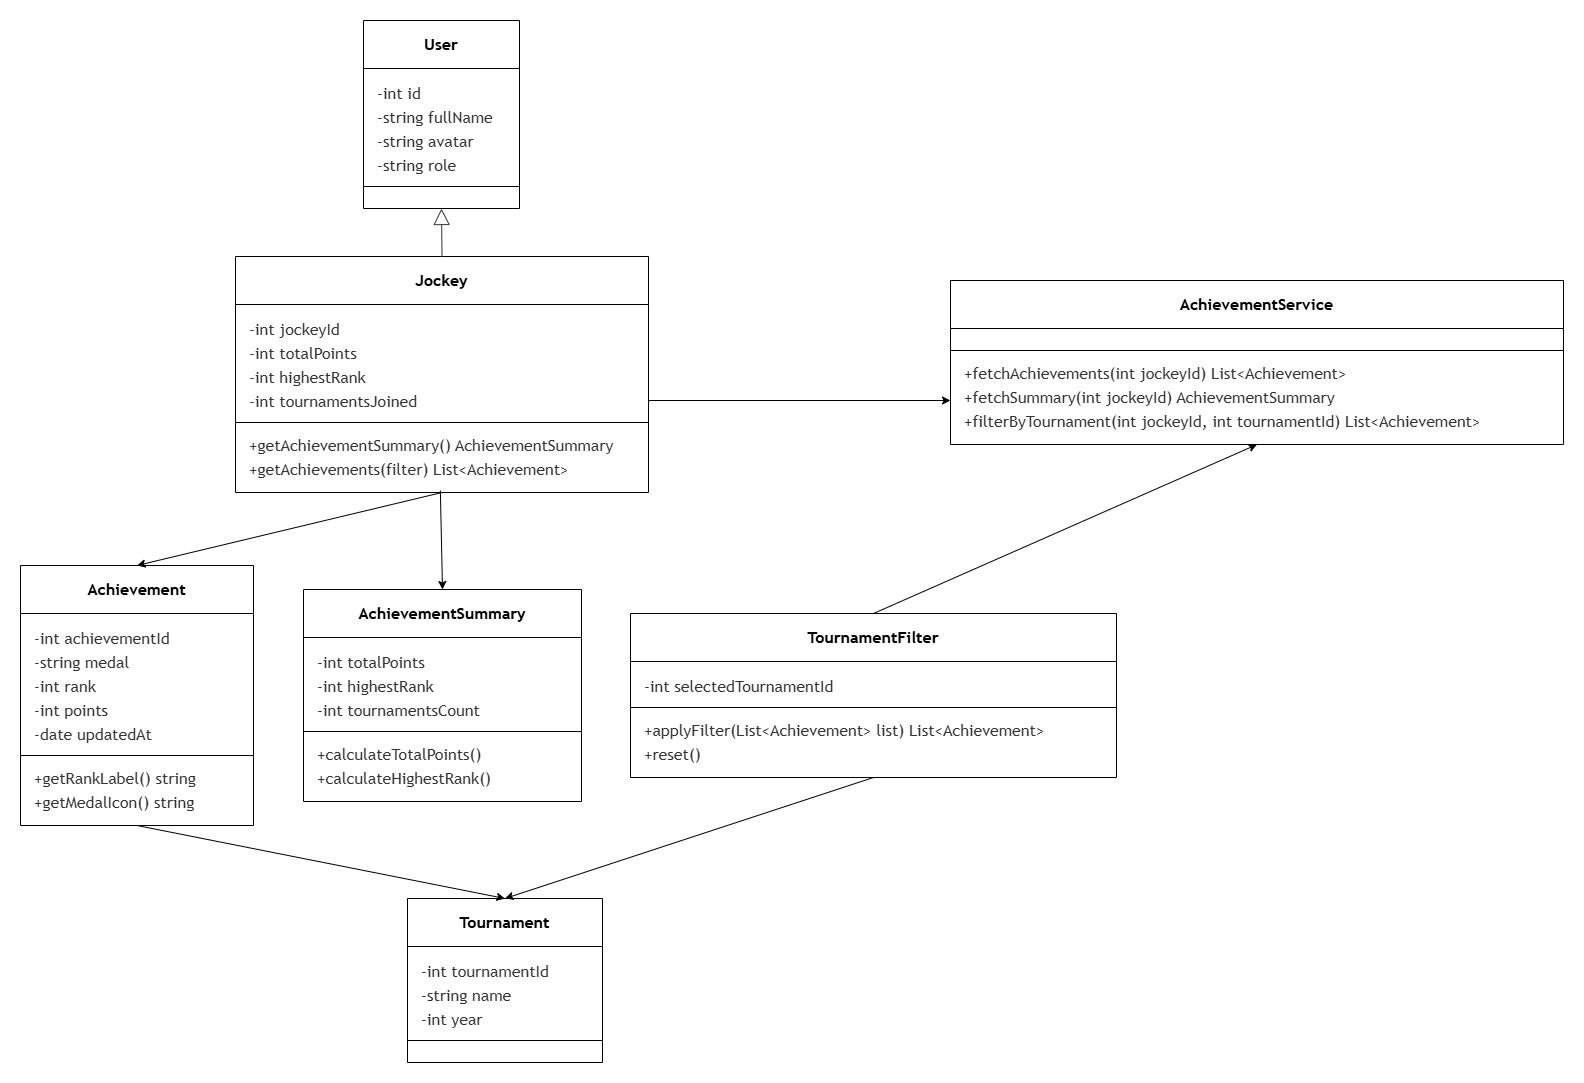
\includegraphics[width=\textwidth,height=0.78\textheight,keepaspectratio]{figures/design/Jockey/classdiagram-achivement_jockey.drawio.drawio.png}
    \caption{Achievements Class Diagram}
    \label{fig:jockey_achievement_class_diagram}
\end{figure}

\subsubsection{Sequence Diagram}

\begin{figure}[H]
    \centering
    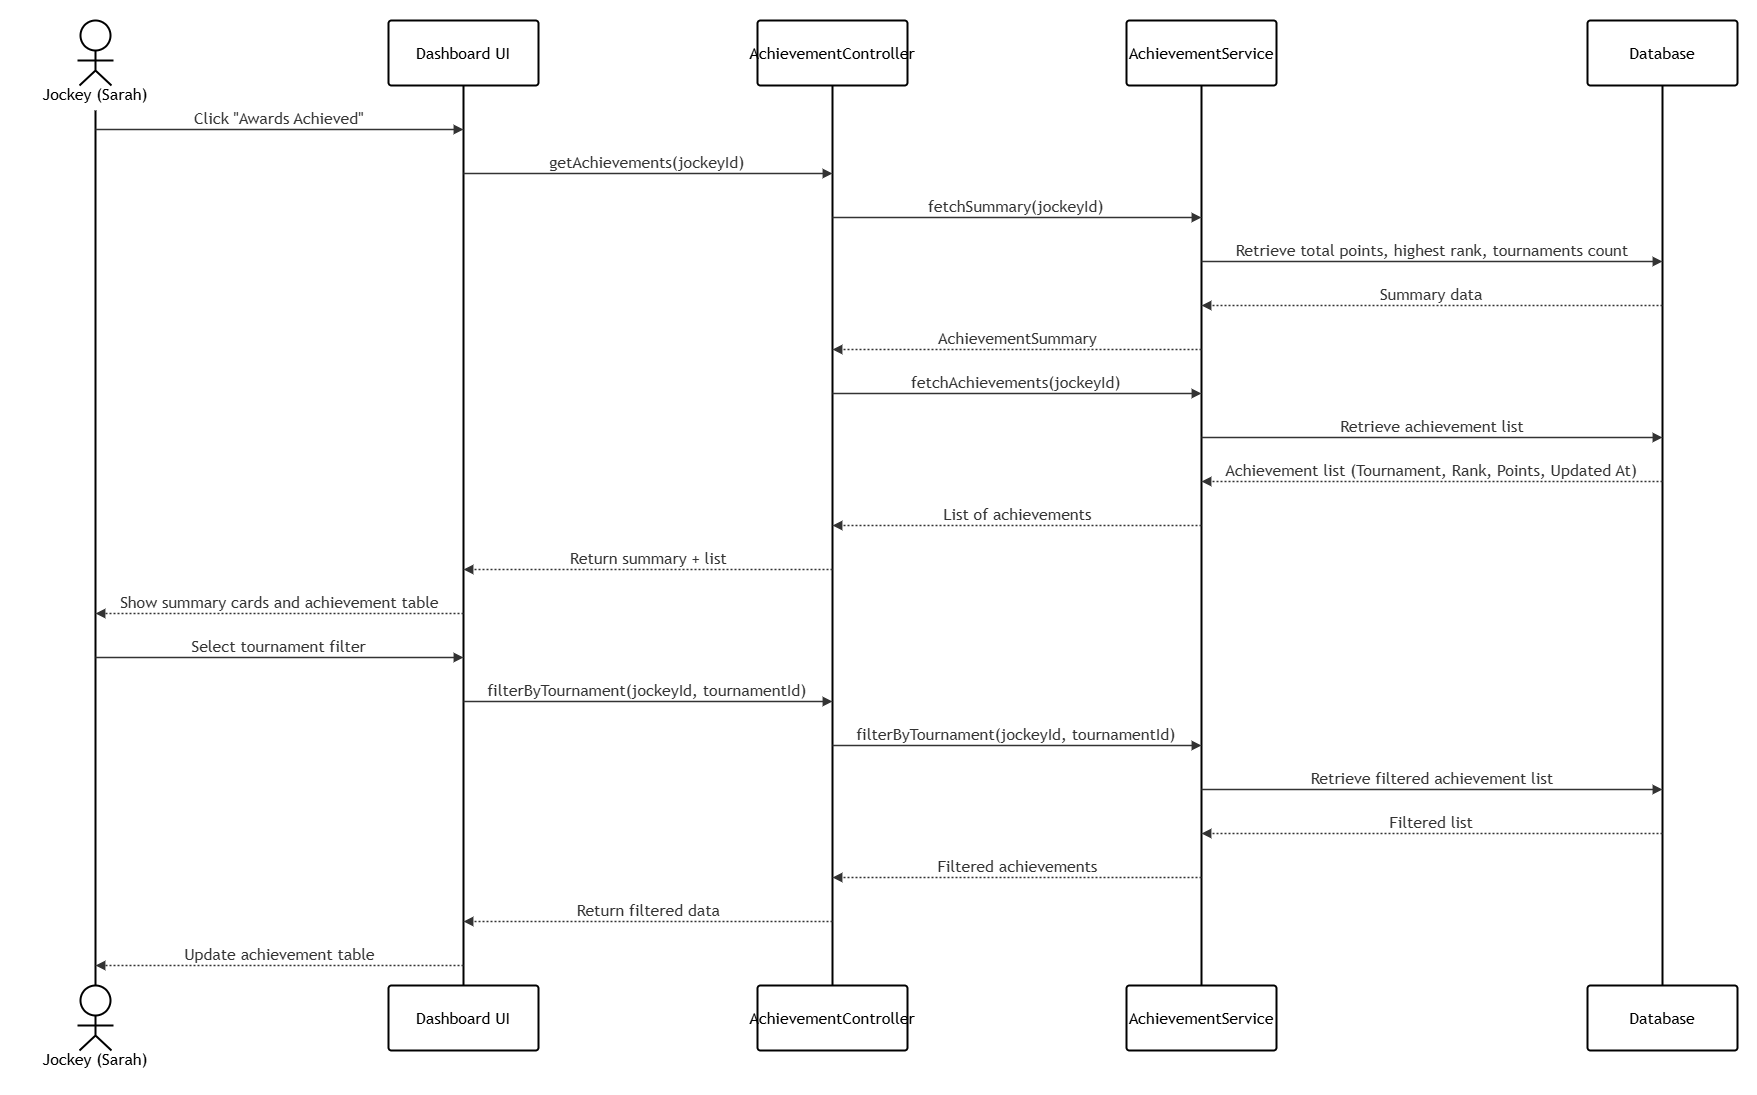
\includegraphics[width=\textwidth,height=0.78\textheight,keepaspectratio]{figures/design/Jockey/sequence-achivement_jockey.drawio.drawio.png}
    \caption{Achievements Sequence Diagram}
    \label{fig:jockey_achievement_sequence_diagram}
\end{figure}

\subsubsection{Class Specification}

\begingroup
\small
\setlength{\tabcolsep}{3pt}
\begin{longtable}{|>{\raggedright\arraybackslash}p{0.16\textwidth}|>{\raggedright\arraybackslash}p{0.30\textwidth}|>{\raggedright\arraybackslash}p{0.14\textwidth}|>{\raggedright\arraybackslash}p{0.25\textwidth}|}
\caption{Achievements class specification}
\label{tab:jockey_achievement_class_spec} \\
\hline
\tableHeader
\textbf{Class} & \textbf{Attributes / Methods} & \textbf{Type} & \textbf{Description} \\
\hline
\endfirsthead
\hline
\tableHeader
\textbf{Class} & \textbf{Attributes / Methods} & \textbf{Type} & \textbf{Description} \\
\hline
\endhead
User & id, fullName, avatar, role & entity & Base account class inherited by \texttt{Jockey}, providing shared identity attributes for the achievements feature. \\
\hline
Jockey & jockeyId, totalPoints, highestRank, tournamentsJoined, getAchievementSummary(), getAchievements(filter) & entity & Extends \texttt{User}; stores cumulative performance statistics and delegates achievement retrieval to \texttt{AchievementService}. \\
\hline
Achievement & achievementId, medal, rank, points, updatedAt, getRankLabel(), getMedalIcon() & entity & Represents a single achievement record earned by the jockey in a tournament, with helper methods for display formatting. \\
\hline
Achievement\allowbreak{}Summary & totalPoints, highestRank, tournamentsCount, calculateTotalPoints(), calculateHighestRank() & DTO & Aggregates the jockey's overall performance statistics shown as summary cards on the achievements page. \\
\hline
Achievement\allowbreak{}Service & fetchAchievements(jockeyId), fetchSummary(jockeyId), filterByTournament(jockeyId, tournamentId) & service & Handles all data retrieval for achievements, including full lists, summary aggregation, and tournament-based filtering. \\
\hline
Tournament\allowbreak{}Filter & selectedTournamentId, applyFilter(list), reset() & service & Applies a tournament filter to the achievement list and supports resetting the filter to show all achievements. \\
\hline
Tournament & tournamentId, name, year & entity & Provides the tournament context for each achievement record and supports filter selection on the achievements page. \\
\hline
Dashboard\allowbreak{}UI & getAchievements(jockeyId), filterByTournament(jockeyId, tournamentId) & boundary / UI & Renders the achievements summary cards and table, and updates the view when the jockey selects a tournament filter. \\
\hline
Achievement\allowbreak{}Controller & getAchievements(jockeyId), filterByTournament(jockeyId, tournamentId) & controller & Coordinates between the UI and \texttt{AchievementService} to fetch full or filtered achievement data for the jockey. \\
\hline
\end{longtable}
\endgroup

